\numberwithin{equation}{section}
\numberwithin{figure}{section}
\numberwithin{table}{section}

The rig design is based on the design criteria given in the competition guidelines. Mobility, functionality, versatility, stability, and safety have been the main concerns while designing the rig. The focus has been on having a hoisting and rotary system with high precision and functionality to ensure an efficient drilling operation. Using equipment that is already available in the university workshop has been a key concern to make the project as cost efficient as possible.

\subsection{Rig Structure}
Steel has been chosen as construction material for the main structure of the rig to ensure rigidity and stability. It also has the benefit of being cost efficient and easily accessible. Aluminum profiles were also considered, but were not chosen due to its high cost. The weight of the rig construction will be 100kg, using steel as construction material.    

The height of the drilling rig was estimated based on the rock sample height (0.60 m) and the total length of the assembled drill string. Since no making or breaking of connections will be done, the length of the drill string will be customized to drill through the block in one go. The total length of the drill string accommodates for a full length of drill pipe (0.914 m), bottom hole assembly and bit. Refer to figure (\ref{fig:SideViewUp}), (\ref{fig:SideViewUpDim}) and (\ref{fig:FrontView}) for illustration and dimensions of the rig structure. 
\begin{figure} [H]
\centering
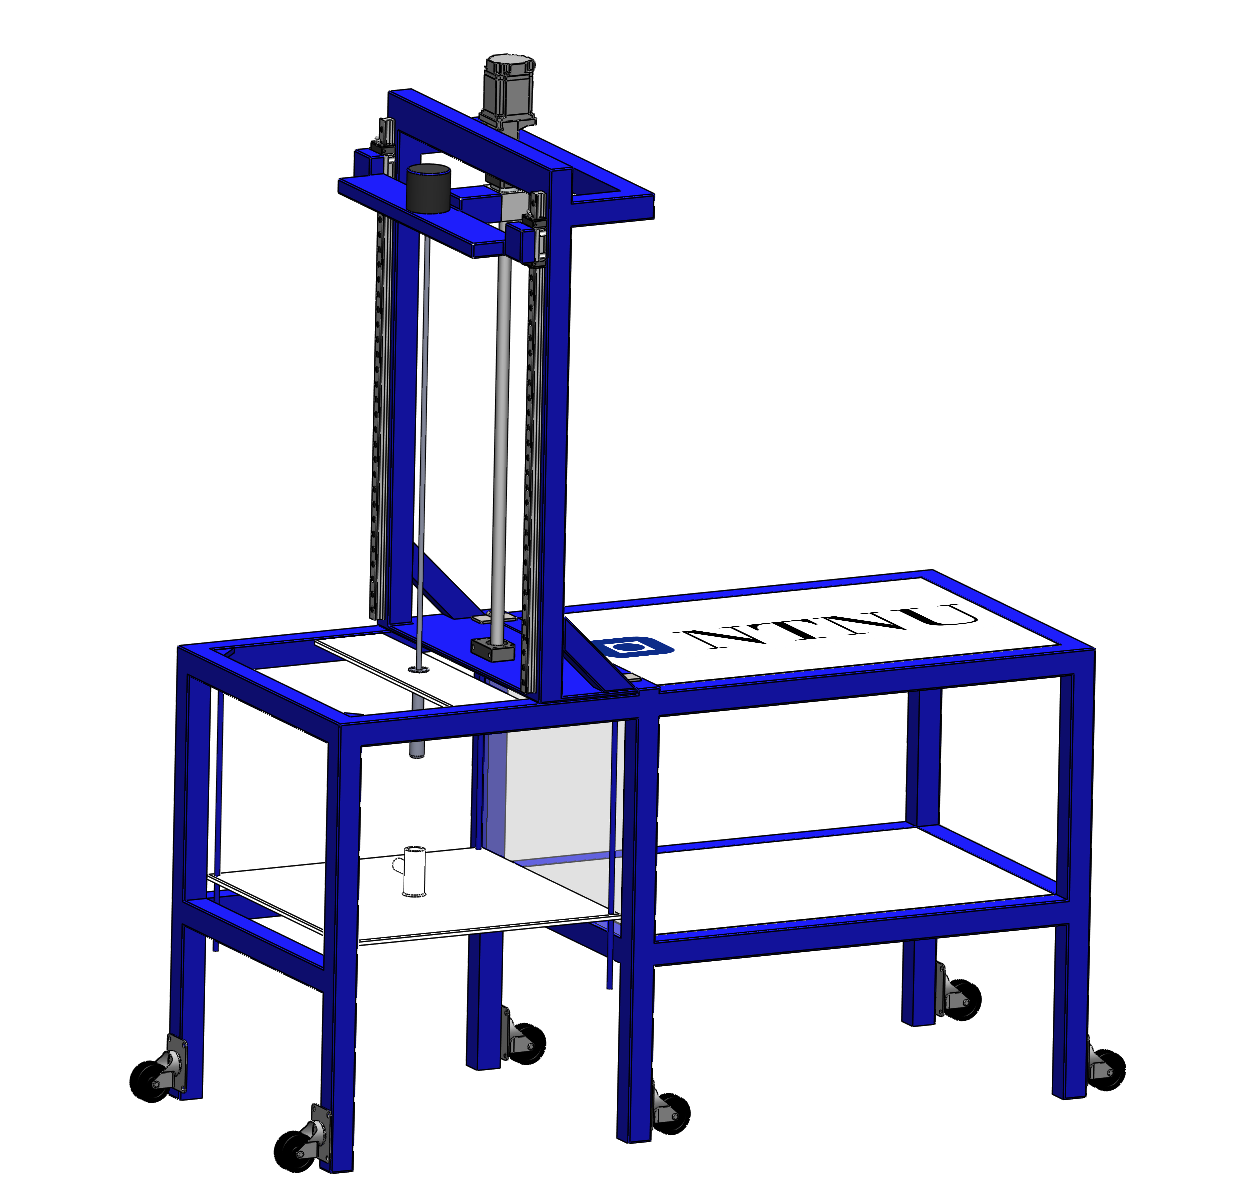
\includegraphics[width=0.6\textwidth]{figures/SideViewUp.PNG}
\caption{Illustration of the rig rig in upright position}
\label{fig:SideViewUp}
\end{figure}

\begin{figure} [H]
\centering
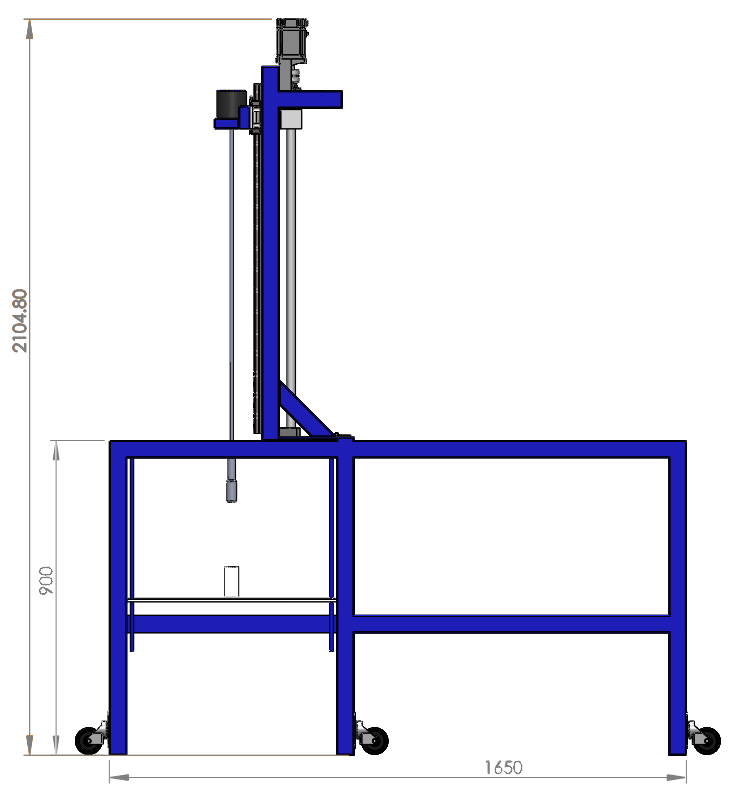
\includegraphics[width=0.6\textwidth]{figures/Sidedimensions.PNG}
\caption{Side view of the rig in upright position (dimensions in mm)}
\label{fig:SideViewUpDim}
\end{figure}


\begin{figure} [H]
\centering
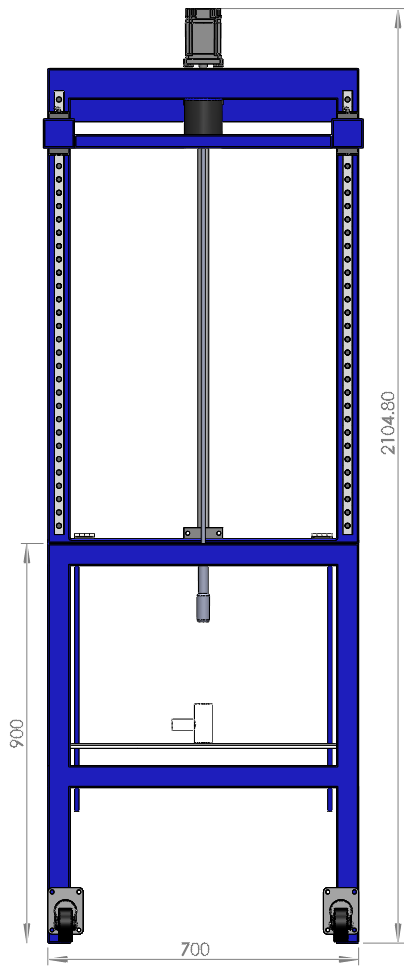
\includegraphics[width=0.3\textwidth]{figures/FrontDimensions.PNG}
\caption{Front view of the rig in upright position (dimensions in mm)}
\label{fig:FrontView}
\end{figure}


Because versatility has been important when designing the rig, the height and width of the structure were chosen to allow for a formation height up 70 cm and width up to 60 cm.

An adjustable steel plate with a thickness of 10 mm, guided by rails, will be lowered down to the formation top. The plate will, together with clamps, keep the formation at bay when drilling. A steel cylinder with a length of 80 mm and an inner diameter of 30 mm will be welded to the plate. It will be centered on the plate and work as a guiding shoe for the bit. Because the steel cylinder imitates the function of a riser, it will be referred to as a riser in the text.

\begin{figure} [H]
\centering
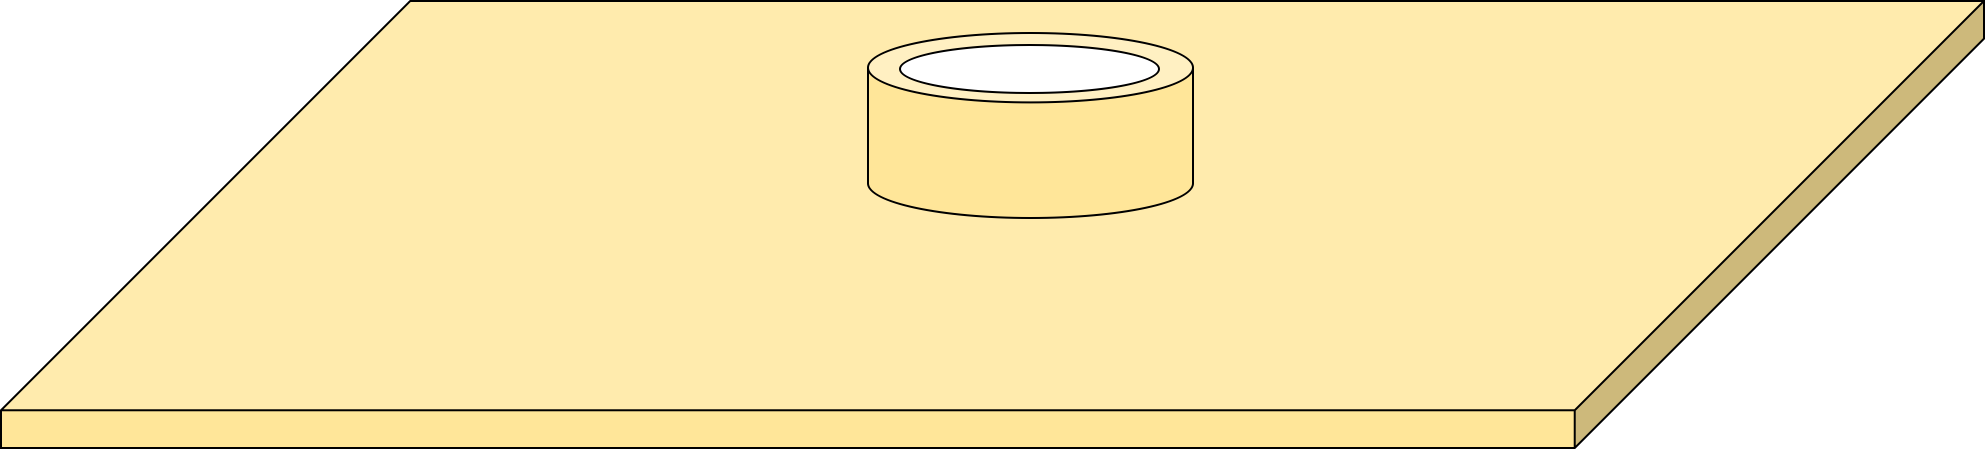
\includegraphics[width=0.6\textwidth]{figures/riser.png}
\caption{Illustration of steel plate and attached riser}
\label{fig:riser}
\end{figure}

A second cylinder with a length of 30 mm and an inner diameter of 10 mm will sit on the top of the BHA. It will consist of two parts: a hanger and a body. The hanger, of length 10 mm, will have an outer diameter larger than the outer diameter of the riser, and the body, of length 20 mm, will have an outer diameter smaller than the inner diameter of the riser. This will make it possible to land the cylinder on the riser.

\begin{figure} [H]
\centering
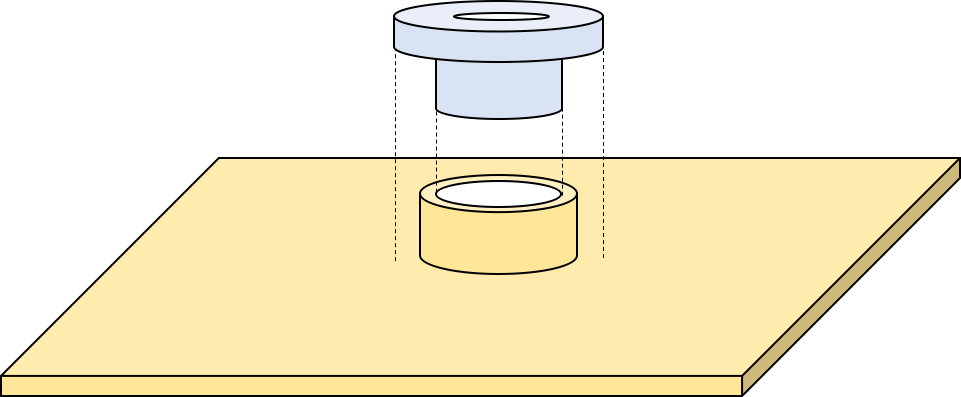
\includegraphics[width=0.6\textwidth]{figures/surfacestabilizer.png}
\caption{Illustration of steel plate, riser and surface stabilizer}
\label{fig:surfacestabilizer}
\end{figure}

As the drill string moves downwards, the cylinder will be guided into the riser and the hanger will make sure it stays inside the riser. This will provide stability for the drill string once the BHA and bit have entered the formation, and will therefore be referred to as a surface stabilizer. The combination of the riser and the surface stabilizer will provide stability during the entire drilling operation. See figure (\ref{fig:conductor}).
\begin{figure} [H]
\centering
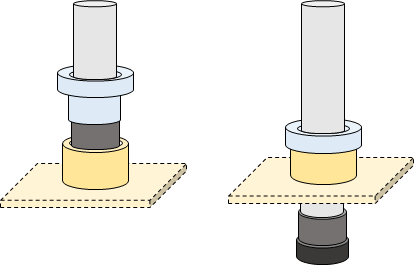
\includegraphics[width=0.6\textwidth]{figures/ConductorStab.png}
\caption{Illustration of riser and surface stabilizer}
\label{fig:conductor}
\end{figure}


A kelly bushing, in the form of a roller bearing, will be attached to the drill deck floor and serve as a stabilizing element to prevent excessive lateral vibrations and also imitate the actual drilling operation as much as possible. The inner diameter of the roller bearing will be slightly larger than the outer diameter of the drill pipe. The pipe will be guided through the roller bearing before BHA and bit is attached to the string. See figure (\ref{fig:Roller}). This roller bearing can easily be removed if the judges disallow it. 

\begin{figure} [H]
\centering
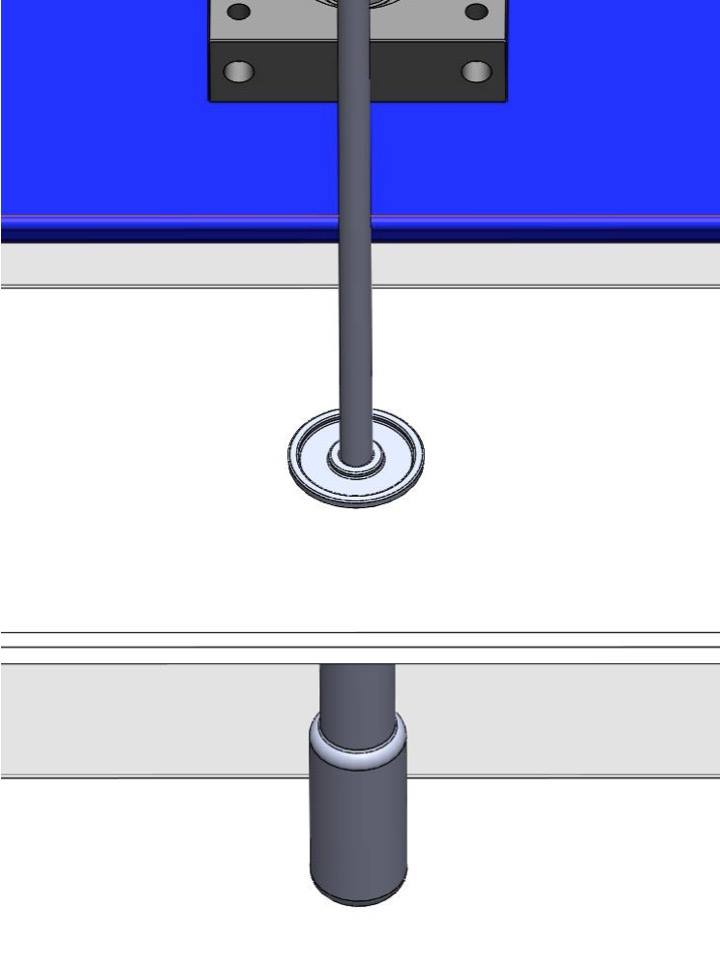
\includegraphics[width=0.5\textwidth]{figures/Roller.jpg}
\caption{Illustration of drill string running through roller bearing}
\label{fig:Roller}
\end{figure}

\subsection{Mobility of Rig}
The drilling rig is designed to easily be moved around, as well as to ensure quick rig up and rig down. Jack up casters are used on each leg to allow for mobility so that the rig can effortlessly be operated by one person. The casters will also make it possible to put the structure down on its steel legs to ensure stability when operating. The derrick is mounted to the rest of the structure by hinges and bolts, and can be folded down for a steady and safe transport. The structure is designed to be able to pass through a standard doorway, with a folded down height and width of 1.266 m and 0.7 m, respectively. Figure (\ref{fig:SideViewDown}) and (\ref{fig:SideViewDownDim}) illustrate the folded position of the rig with dimensions. 

\begin{figure} [H]
\centering
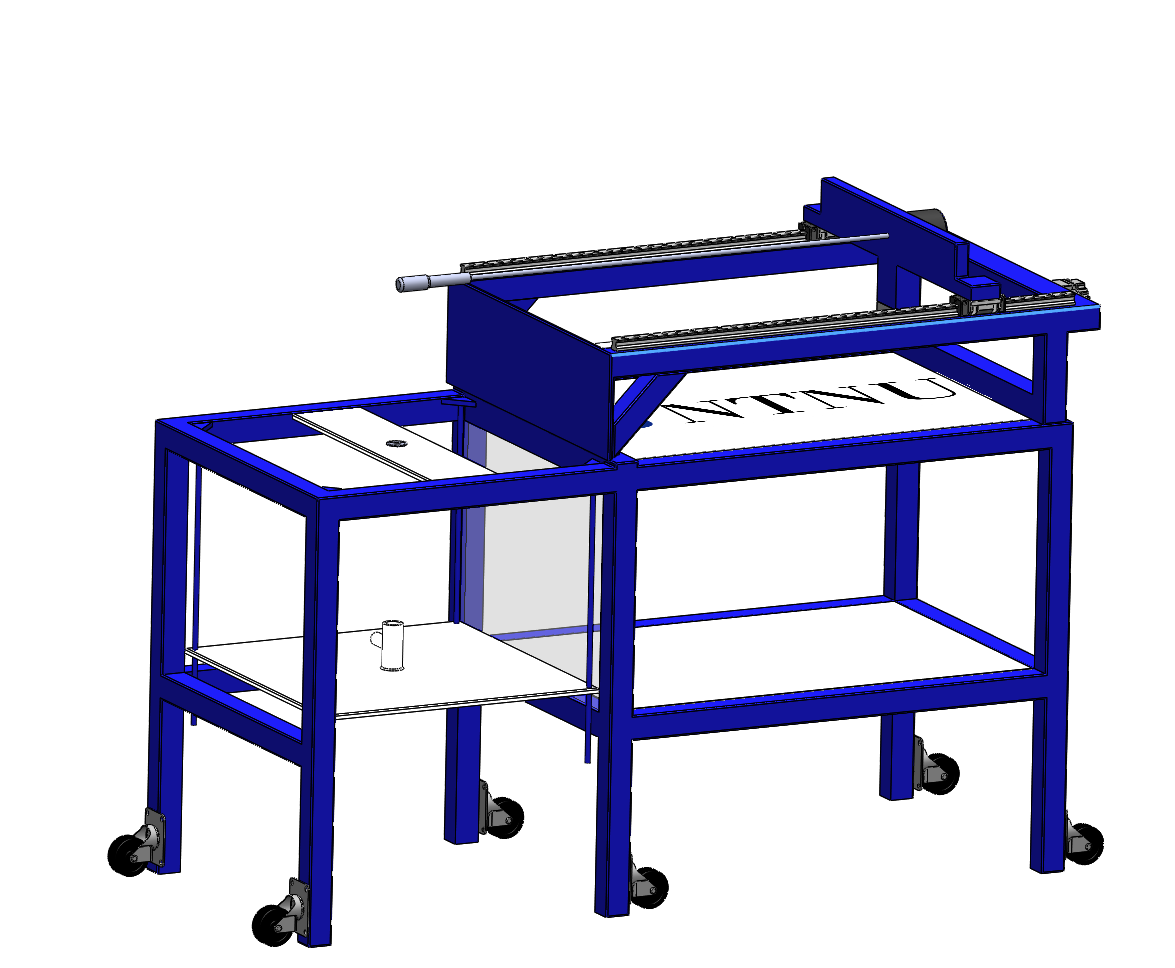
\includegraphics[width=0.7\textwidth]{figures/SideViewDown.PNG}
\caption{Illustration of the rig in folded position}
\label{fig:SideViewDown}
\end{figure}


\begin{figure} [H]
\centering
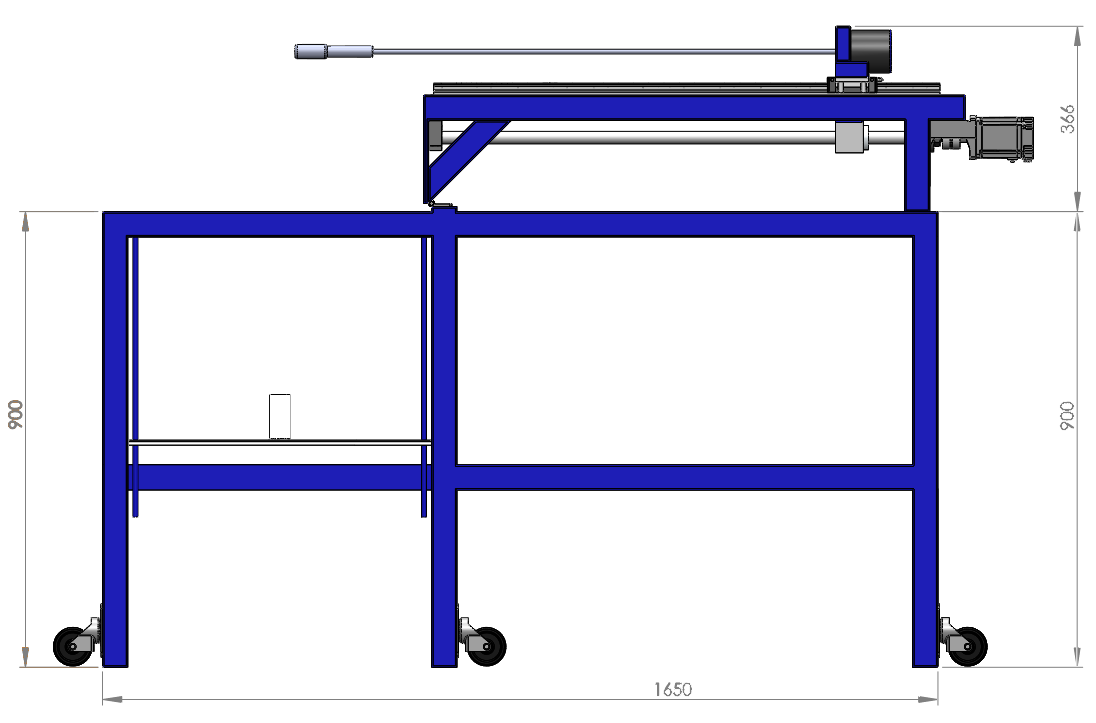
\includegraphics[width=0.7\textwidth]{figures/SideDimensionDown.PNG}
\caption{Side view of the rig in folded position (dimensions in mm)}
\label{fig:SideViewDownDim}
\end{figure}




\subsection{Hoisting System}
The hoisting system provides vertical movement of the travelling block assembly to perform the drilling operation. A traditional hoisting system with drawworks was considered, but found to be inapplicable because of its complexity and lack of precision. Unlike the traditional situation, this hoisting system needs to be able to push down the string to apply weight on bit. Rack and pinion drive was weighed against ball screw drive, where the ball screw was selected due to a higher accuracy and step resolution. 

\begin{figure} [H]
\centering
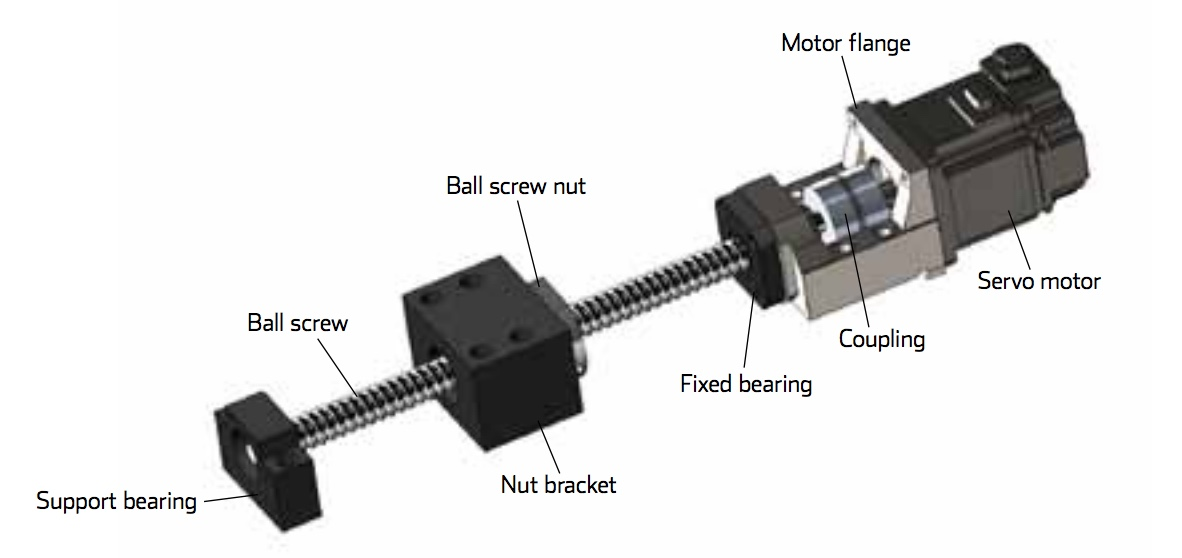
\includegraphics[width=0.7\textwidth]{figures/CompleteBS.jpeg}
\caption{Illustration of the complete ball screw package (MBA20-E-Comp) that will be used for the hoisting system \cite{aluflex}}
\label{fig:ballscrew}
\end{figure}

A 24 V DC-motor will drive the ball screw which converts rotational energy to linear motion. Because of the mechanical advantage of the ball screw, this motor will not need a high torque-output, but rather a high RPM. The power calculations for the motor will be performed in section 4.3.

A linear roller guide system will be combined with the ball screw to provide stable vertical motion and eliminate horizontal movement.

\begin{figure} [H]
\centering
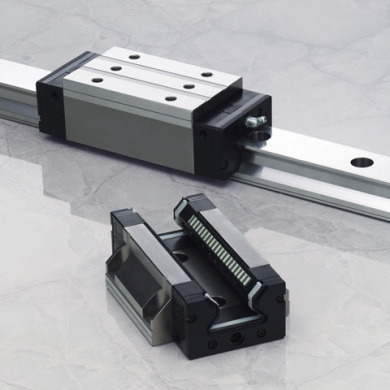
\includegraphics[width=0.5\textwidth]{figures/rollerguide.jpg}
\caption{Illustration of linear roller guide for hoisting system \cite{pic_rail}}
\label{fig:rollerguide}
\end{figure}


The linear roller guide is a low friction system which will ensure accurate WOB-measurements. It will also provide stability and high rigidity to the structure. The lead of the ball screw, together with motor selection, makes it possible to decide the hoisting speed and accuracy. An accurate hoisting system, with a low-lead ball screw, facilitates small incremented and precise weight on bit changes. 



\subsection{Rotary System}
The main function of the rotary system is to provide torque to the bit through the drill string. Both rotary table and top drive system have been considered, where the top drive system was chosen as the best solution. Even though the rotary table system would have made it easier to design the circulation system, the top drive system contains less components and provides higher power efficiency since the motor is directly connected to drill pipe. 

The top drive system will consist of a 24 V DC-engine, and the required motor power will be calculated in section 3.5. A swivel will also be included to implement the circulation system. 



\subsection{Drill String Design}
The drill string consists of a drill pipe and a BHA. The combined length of the drill string will be kept as short as possible to mitigate vibrations. It is stated in the competition guidelines that at least one length of drill pipe (91.4 cm) must be used. The BHA will be optimized to fit both the sensors and stabilizer, and will therefore have a length of 80 mm. Since the surface stabilizer has a length of 30 mm, the stabilizer in the BHA will be limited to a length of 60 mm to fulfill the requirements in the guidelines. The drill bit will have a maximum length of 64 mm.    

One of the main judging criteria is the verticality of the borehole. Stabilizers will be used to control the hole deviation and counteract vibrations. Several types of stabilizers have been considered, shown in tabel (\ref{tab:evastab}), where the welded stabilizers were chosen as the best suited solution due to their simplicity. 


\begin{table} [H]
    \centering
    \caption{Evaluation of Stabilizers}
    \begin{tabular}{p{2cm}|p{3cm}|p{3cm}|p{3cm}}
        Type & Description & Pros & Cons \\ \hline \hline
        Integral blade & Blades are an integral part of the tool body & No risk of leaving components into wellbore & Difficult to machine, expensive \\ \hline
        Welded blade & Blades are welded on to the tool body & Easy to make, cheap & Weak points in welding  \\ \hline
        Sleeve type & Replaceable sleeve mounted onto the tool body & Replaceable & Needs threading  \\ \hline
        Non-rotating & Rubber sleeve – remains stationary while the string rotates & Less wear on the blades, good for hard formations & Difficult to make, expensive  \\
    \end{tabular}
    \label{tab:evastab}
\end{table}


The main body of the BHA will have an outer diameter of 22.9 mm. To minimize frictional forces, the stabilizer blades will have an outer diameter of 28 mm, which is slightly smaller than the diameter of the wellbore being drilled. Spiral blades will be used, and the distance between the blades will provide enough space to transport cuttings and avoid pressure build-up in the wellbore. An illustration of the stabilizer is shown in figure (\ref{fig:stabilizer})

\begin{figure} [H]
\centering
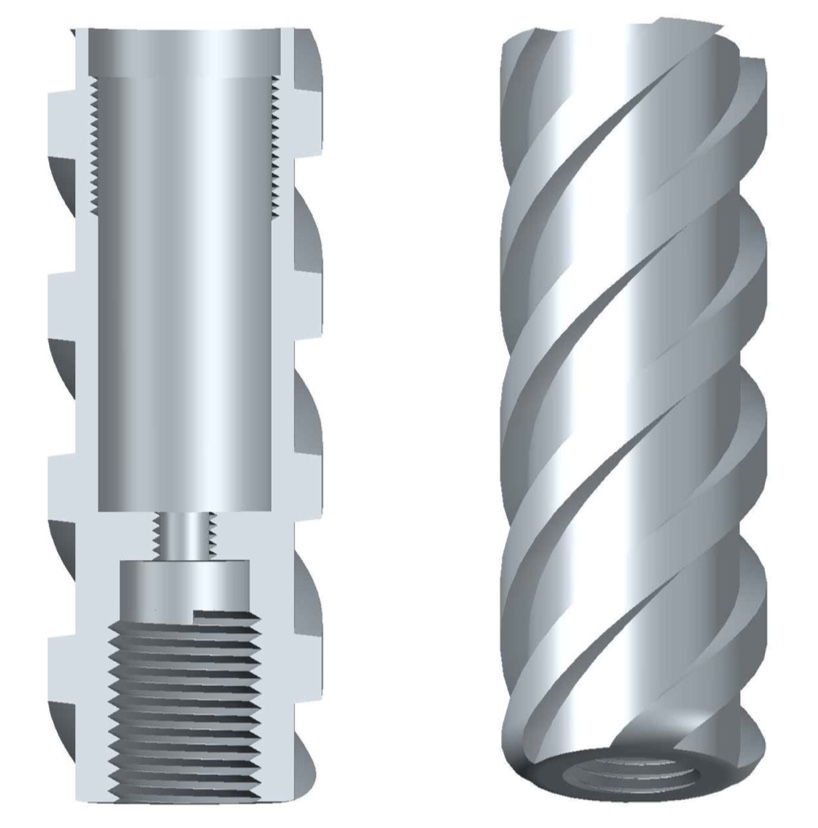
\includegraphics[width=0.5\textwidth]{figures/Stabilizer.jpeg}
\caption{Illustration of the stabilizer, showing a side cut on the left hand side}
\label{fig:stabilizer}
\end{figure}



Hydraulic connections will be used as tool joints between the BHA and the pipe as well as between the pipe and the swivel. The internal pressure in the drill string may exceed 40 bar to increase the internal stiffness in the pipe. Hydraulic connections have been chosen because of this high pressure felt by the drill string during operation. 